% This is samplepaper.tex, a sample chapter demonstrating the
% LLNCS macro package for Springer Computer Science proceedings;
% Version 2.20 of 2017/10/04
%
\documentclass[runningheads]{llncs}
%
\usepackage{graphicx}
% Used for displaying a sample figure. If possible, figure files should
% be included in EPS format.
%
% If you use the hyperref package, please uncomment the following line
% to display URLs in blue roman font according to Springer's eBook style:
% \renewcommand\UrlFont{\color{blue}\rmfamily}

\usepackage{csquotes}
\usepackage{longtable}



\begin{document}

\section*{Correction notice}
In Section \ref{quality}, it is indicated that the model with the highest $C_v$ coherence score was chosen for analysis. Unfortunately, it turned out that the wrong model was manually loaded for analysis. As explained in Section \ref{parameters} the algorithm used in this paper has the option for it's user to specify a so-called random state: a seed that the model uses for the required randomness. While processing the results from the model search phase, two random states got mislabeled, resulting in the wrong model being selected for analysis. The number of topics is equal between the two models, but the chosen seed was different and so was the coherence. The best model had a $C_v$ of 0.517, while the wrongfully chosen model scored 0.504.  

In terms of topics, the two models differ in various ways. Comparing the two, 26 of the topics overlap in a one-to-one relation. For the other 10 topics there are differences. Some examples are given, from the perspective of the 'right' model, i.e., the one with a higher $C_v$ coherence: The two topics that were labelled as \textit{Social networks} and \textit{Social media use} seems to have 'merged' into one, so have the topics of \textit{Cryptography} and \textit{Signature}. Additionally, this model uncovered a specific topic with terms like \textit{image} and \textit{video} as distinguishing terms, as well as a topic with \textit{blockchain}, \textit{voting}, and \textit{payment}. These terms were previously contained in different topics. On the other hand, the topics of \textit{Big data}, \textit{Office design} and \textit{Application security} are not uncovered as such by the 'right' model. This once again signals the somewhat arbitrary nature of a topic model. As mentioned in Section \ref{search}, every model we choose to analyse is one of various possible models with a different representation of the underlying documents.

Because this type of modelling is very susceptible to changes in factors like the random state, the discussion in Section \ref{discussion} already explicitly avoids drawing conclusions that would not be generalizable to different models. At a first glance, partly repeating the analysis of Section \ref{comparison} shows that the specific relations between communities and topics change as an effect of the new topic model, but the general pattern of some 1-on-1 relations, larger communities covering multiple topics, and differences of which we cannot know the reasons hold. Because the observations in this paper are not on the level of specific patterns in the privacy literature, but mainly on this method's usage and usefulness, all findings remain valid.

 

%
\title{Topical Analysis of Privacy Literature, with an Application on Citation Network Interpretation} % \thanks{Supported by organization x.}}
%
\titlerunning{Topical Analysis of Privacy Literature}
% If the paper title is too long for the running head, you can set
% an abbreviated paper title here
%
\author{Joost Gadellaa}
%
\authorrunning{J.F. Gadellaa}
% First names are abbreviated in the running head.
% If there are more than two authors, 'et al.' is used.
%
\institute{Universiteit Utrecht, Heidelberglaan 8, 3584CS Utrecht
\email{j.f.gadellaa@students.uu.nl}}\\
%
\maketitle              % typeset the header of the contribution
%
\begin{abstract}
Privacy is a versatile field of research, studied in a multitude of disciplines. A novel way to explore how research concepts like these are embedded in scientific literature is through the use of topic models. This study aims to investigate the usefulness of such modelling techniques. We use a latent Dirichlet allocation (LDA) topic model to analyse the title, abstract and keywords of 83,159 works in the research field of privacy, evaluating the model both on its own as well as in comparison to a previously made citation network analysis. We show that, although the resulting topic model can be meaningfully labeled, interpretation yields little insights. When comparing the model to the citation network analysis, remarkable similarities between the resulting classifications of these very different methods show. However, many methodological caveats pose a threat to conclusion validity, and computational costs limit possibilities for additional exploration. This method needs further research in order to generate insights, instead of just being an accurate representation of the data. 
\keywords{Privacy \and Topic model \and LDA \and Privacy \and Network Analysis \and Bibliometrics}
\end{abstract}
%
%
%
\section{Introduction}
Privacy is a broad concept studied in various disciplines of science. The scientific discussion about the topic originates when the “Right to be let alone” was recognized “in common law, in its eternal youth, […] to meet the demand of society” \cite{warren_right_1890}. Since then, it has become an increasingly multidisciplinary concept studied by medicine, psychology, engineering, computer science, and law scholars amongst others. In a time when data-driven technological possibilities are developing fast, people are more and more concerned about their personal privacy \cite{kokolakis_privacy_2017}. The topic seems more pressing than ever. 

The scattered nature the privacy research field creates a need for mapping studies. Understanding privacy’s scientific discourse is essential to aid literature reviews, facilitate interdisciplinary sharing of knowledge, identify lacunae, and develop policy supporting the research field's development \cite{noyons_bibliometric_1999}. Future research paths are hard to identify and a clear direction more challenging to articulate without a coherent connection between the different theoretical understandings, practical artifacts, and empirical models. 

A relatively novel approach to conduct mapping studies is through the usage of topic models. Topic modeling is an area of unsupervised machine learning in which text corpora are modeled by means of their latent topics: groups of co-occurring words associated with a single theme \cite{dimaggio_exploiting_2013}. This method uncovers similarities between documents in the corpus and describes the documents using these relations without a need for categorization by human annotators. This method has found its way from computer science and linguistics to less technical fields like communication research \cite{maier_applying_2018}, fisheries science \cite{syed_narrow_2018}, and journalism \cite{jacobi_quantitative_2016}. Topic models have also shown some promising results for the purpose of automatic discovery of sub-fields in scientific literature \cite{mimno_bibliometric_2006}, which will be the focus of this analysis.

Taking an approach strongly focused on methods, this analysis’ goal is to explore the value of topic models for the use of understanding privacy’s scientific discourse. The main research question is: How can topic models contribute to our understanding of privacy’s embedding in the scientific literature. Two sub-goals will be introduced below: creating and exploring a topic model, and comparing it to a citation network analysis of the same data.

The first goal is to create a coherent topic model that captures the diverse nature of privacy as a scientific research field. Using this model, we might be able to answer exploratory questions on the existence of different sub-fields and relations between them. Special attention will be on the method design. Although the existence of easy-to-use open-source libraries like Gensim \cite{rehurek_gensimpython_2011} and Mallet \cite{mccallum_malletmachine_2002} have enabled many scholars to employ topic models in novel ways, the method’s underlying complex statistical nature may put scientific rigor at stake when not utilized properly. Researchers often treat these kinds of algorithms as ‘black boxes’, without thoroughly exploring and tuning underlying parameter values \cite{chen_survey_2016}. Therefore, the creation of a topic model for analysis must not be secondary to its interpretation.

The second goal is to compare the then discovered topic model to a network analysis of the same data by Van Dijk \cite{van_dijk_pillars_nodate}. Their quantitative analysis and its translation to qualitative identification of the theoretical foundation of privacy as a research field is a prime example of what this kind of research can contribute. Seeing what similarities and differences between a classification based on citation communities and one on latent topics exist could tell us more about the value of these methods. The topic model might additionally be used to interpret or label citation communities more accurately or objectively. Above all, it stimulates discussion about the research field and the application of novel methods.

This paper will explore how topic models can contribute to our understanding of privacy’s embedding in the scientific literature. We will elaborate on the methodology in Section \ref{Methods} including a short non-technical description of LDA topic models. After a valid model has been found, it will be interpreted through its topic labels, topic correlation, and a comparison to the citation network analysis in Section \ref{results}. Section \ref{discussion} will reflect on the research goals and the results’ consequences for the research question and possible directions for future research.


\section{Methods} 
\label{Methods} 
\subsection{Latent Dirichlet Allocation}
In the context of bibliometric analyses and in general, one of the most frequently used topic models is the Latent Dirichlet Allocation (LDA) \cite{blei2003latent}. This generative probabilistic model uses the frequencies of words in the documents to uncover latent topics and assign every document a distribution over these topics. LDA is a mixed membership model, which means that documents are seen as part of multiple topics in different proportions. This makes it particularly suitable for exploratory and descriptive analyses \cite{elgesem2015structure}. By capturing the heterogeneity of research topics that a specific paper can belong to, LDA overcomes the limitations of other topic models like Latent Semantic Indexing (LSI) \cite{dumais1994latent} and pLSI \cite{hofmann1999probabilistic}; besides the main topic it is assigned to, a paper covers multiple topics in different proportions \cite{syed_full-text_2017}. It is important to note that LDA is a bag-of-words (BOW) model, meaning it does not consider the order of words, just their presence and count within a document. Although this is a heavy simplification from how humans understand text, it is well-founded for the purpose of uncovering latent structures \cite{blei_dynamic_2006}.

\subsection{Data retrieval}
\label{retrieval}
For this analysis, bibliometric data on the field of privacy gathered by Van Dijk \cite{van_dijk_pillars_nodate} is used and extended. The set consists of 119,710 published works with privacy in their title, abstract, author-specified keywords, or publisher keywords. The data is further filtered on having at least one reference to or from another work in the set. This results in a subset of 83,159 works. This data was extended by querying the Scopus API for the corresponding keywords and abstracts using Pybliometrics \cite{rose2019pybliometrics}. Here, only keywords added by the author(s) were included in the data set to prevent the Topic Model from learning from previous categorizations, be it automatic or human. Only abstracts, in contrast to full texts, are considered for computational feasibility reasons. For large document collections like these, the benefit from the inclusion of more text is negligible \cite{syed_full-text_2017}. Scopus was used because of its high quality and advanced curation of sources to include \cite{baas2020scopus}.

\subsection{Data processing}
\label{processing}
One of this analysis’ main goals is to create a topic model in a reproducible and objective way. As Maier \textit{et al.} \cite{maier_applying_2018} stated, two of the main methodological steps that need to be taken to reach this goal are appropriate pre-processing and adequate selection of model parameters. It is a downside of LDA that these steps can influence results in a significant way and that their order matters \cite{denny2018text}; consecutive steps are dependent on previous results. The follow in appraoch is chosen, closely following recommendations by Maier et al.. 

The first step of pre-processing consists of the cleaning of data. Copyright notices are removed from the abstracts using a regular expression to prevent the topic distribution from being influenced by the organization that published the work. Afterward, we take the following steps in this specific order: Tokenization, converting to lowercase, punctuation removal, stop-word removal, lemmatization and stemming, and relative pruning. 

The sentences are split into a list of words, also known as tokens. Using the Gensim package \cite{rehurek_gensimpython_2011} for Python, this step is easily combined with converting all letters to lowercase and removing punctuation. Converting to lowercase helps to unify the terms, and removing punctuation reduces complexity. This pre-processing step can be considered the removal of uninformative data in the bag-of-words approach used here \cite{scott1999feature}.

All further steps can be considered feature selection, with the overarching goal to only keep those words with distribution patterns that contribute to distinction between topics. This reduction is also essential for the computational efficiency of the later hyper-parameter tuning. The first of these is stop-word removal: Using NLTK’s English stop-word list \cite{bird_natural_2009}, we remove common stop words like \textit{the}, \textit{is}, and \textit{are}. 

After that, it is common practice to stem or lemmatize all words. Stemming is a procedure in which derivational affixes are cut off to reduce all words with the same stem to a common form using several set heuristics \cite{lovins_development_nodate}. We choose lemmatization using WordNet \cite{miller_wordnet_1995} instead, which is less aggressive and enough feature-reduction for English texts \cite{haselmayer2014measuring}. This procedure only collapses inflicted forms to one term instead of many related words. Most importantly, this keeps nouns and verbs separate tokens, closer to the way a human interprets language.

The last of the feature selection steps is relative pruning. This step consists of removing words that either appear in very little or in almost all documents, sometimes referred to as ‘corpus specific stop words’. These words do not contribute to the aforementioned distinctive distribution patterns, and removing them makes model computation less resource-intensive. No systematic studies have been conducted on which percentages of documents should be considered lower and upper-bound, but 1\% and 95\% seem to be the standard \cite{grimmer2013text,denny2018text} and recently, Maier \textit{et al.} showed that such percentages do not decrease model quality \cite{maier_how_2020}. We remove all words that appear in less than 0.5\% or more than 99\%. These percentages are very much on the safe side but still decrease the number of unique terms by around 95\%, enabling the computation of more models during the model search phase.

To illustrate these steps, the beginning of an abstract by Perera \textit{et al.} \cite{perera_designing_2020} is given below. Of these words, none were later removed by relative pruning.

\begin{displayquote}
\textit{“© 2019 Elsevier Inc. Internet of Things (IoT) applications typically collect and analyse personal data that can be used to derive sensitive information about individuals.”}
\end{displayquote}

\begin{displayquote}
\begin{verbatim}
['internet', 'thing', 'iot', 'application', 'typically', 
'collect', 'analyse', 'personal', 'data', 'used', 'derive', 
'sensitive', 'information', 'individual']
\end{verbatim}
\end{displayquote}

\subsection{Parameter tuning}
\label{parameters}
After cleaning the documents, several of LDA’s model parameters have to be defined. Much of our method for finding the optimal model is based on Syed \textit{et al.} \cite{syed_narrow_2018}, who performed a very similar analysis on fisheries science literature. First and foremost, the optimal number of topics ($K$) has to be found. Setting this value too low will result in topics that are too broad to be meaningful, but setting it too high can create semantically meaningless topics that should have been combined \cite{syed_full-text_2017}. In some topic model applications, there are reasons to infer the ‘right’ number of topics from theory or the analysis’ goals. Still, in most cases, the optimal number has to be discovered by generating different models and measure their quality according to a certain metric. There is no ‘true’ number, just a number that produces fitting results according to a chose evaluation metric. The metric of quality for which the model is optimized will be discussed in the next section. 

Apart from the number of topics, the Dirichlet prior distribution on the topic probabilities within documents ($\alpha$) and on the word probabilities within topics ($\eta$) have to be set. The most important choice here is if the topics are expected to have an equal probability of being assigned (a symmetrical prior) or not (an asymmetrical prior). Since in text corpora like these, it is to be expected that some topics are less common than others, an asymmetrical prior is preferred \cite{wallach_rethinking_nodate,syed_exploring_2018}. Gensim’s ‘online’ LDA algorithm \cite{hoffman_online_2010} can use the Newton-Rapson method \cite{huang_maximum_2005} to learn these priors from the data. The technical details of this algorithm are beyond the scope of this analysis, but the relevant effect is that finding the most appropriate priors is not done through an additional dimension in our grid search, saving computation time. 

If computational resources allow for it, the random state, the number of passes through the corpus during training, and the number of iterations for inferring the topic distribution should also be tuned. This is not necessary for each level of $K$, but the convergence profile might differ between versions with different parameters. Currently, no more sophisticated methods than a grid search exist for these parameters. The random state has to be varied to prevent falling into a local minimum \cite{boyd-graber_care_nodate}. In this analysis, we will start with two random states and add more when the grid search has narrowed the possible values for other variables down to a computationally manageable level. Exact values are specified in the accompanying code repository\footnote{https://github.com/JoostGadellaa/Topical-Analysis-of-Privacy-Literature} for reproducibility purposes.

\subsection{Measuring of model quality}
\label{quality}
Any hyper-parameter optimization procedure needs a metric to optimize for. Perplexity \cite{blei2003latent,scott_recursive_2013}, a measurement of goodness of fit on held-out data, is often used for this purpose, but there is no evidence that a good fit aids the interpretability of a topic model by humans\cite{boyd-graber_care_nodate}. Worse still, perplexity might negatively correlate with human judgments of goodness of fit \cite{chang_reading_nodate}. Röder \textit{et al.} \cite{roder_exploring_2015} systematically explored alternatives, and found the combined measure of $C_v$ coherence to show the highest correlation with human understanding on a large variety of test data. This measure is based on the idea that topics have a higher quality when it's top words are more related. Again building on and thorough exploration of alternatives in a similar context by Syed \cite{syed_topic_2019}, we adopt $C_v$ as our measurement of model quality.

\subsection{Topic labeling}
\label{label}
The final part of our topic-model pipeline consists of labeling the topics uncovered by the algorithm. Although human labeling introduces a degree of subjectivity to the process, it is necessary for understanding and reasoning about the obtained model. With automatic methods, like selecting and filtering the most frequent words with feature selection techniques, the downside occurs that the results can be too general and do not account for semantic relationships between words. For example, frequent words can be \textit{red, white} and \textit{blue}, but the best descriptor for this topic would be \textit{colours}. Sometimes, external sources are used for a more semantic approach. Although different algorithms have been developed, they are seldom validated, let alone compared in a structured and rigid manner. As long as the introduced subjectivity is kept in mind during the result evaluation, manual labeling is still the most pragmatic option.

The labeling will be done by two annotators, who separately review each topic’s top-words, the most representative papers per topic (i.e., documents for which the topic distribution has the highest proportion of the current topic), and a visualization using LDAvis \cite{sievert2014ldavis}. The latter serves to judge relative differences in word frequency and add context.


\section{Results}
\label{results}
\subsection{Processed data}
Since Van Dijk’s \cite{van_dijk_pillars_nodate} query of literature mentioning privacy, 126 works have been retracted or otherwise removed. Of the 83,033 works left, 24,982 are without keywords, of which 3534 without abstract. Inspecting a sample shows that these are primarily complete books and conference introductions. 67 works are missing just abstract but have keywords. All documents without abstract are removed since the lack of data would not allow us to properly assign these works a distribution of topics. We don’t have a reason to believe this removal causes bias. Copyright notices were removed with a custom regex available in the code. The above-described relative pruning steps reduced the number of terms from 75148 to 2421; 96.78\% of words occurred too little or too often to contribute to the discovery of latent topics. It is noteworthy that the term \textit{privacy} was not removed, while it is the keyword upon which the papers were selected. This turned out to be because more than 1\% of documents were added to the database because \textit{privacy} was in the keywords added by the publisher. These publisher keywords were not included in this analysis, as described in Section \ref{retrieval}.

\subsection{Model search}
\label{search}
An initial grid search was performed on models with a number of topics ($K$) between 1 and 361. The steps between the different values were based on the power function $x^2$ (1, 4, 9, 16, etc.). This sequence was chosen ad-hoc after some exploratory model generation showed covariance measurements to be less sensitive to changes in topic numbers in the higher regions. The first search across two random states showed that covariance was maximal somewhere between 25 and 49. The search was then deepened to include a total of four random states and additional values for $K$ in between the values in the original sequence. Further exploration of interactions between variables, as described in Section \ref{parameters} was not possible: the current model search already took many days on a regular PC. Nevertheless, the most important variables could be varied in a structured manner, generating a total of 56 models to evaluation.

Most models in this range had a $C_v$ value between 0.32 and 0.49, showing a clear pattern where $C_v$ scores increased sharply for the initial 'increase' in $K$. After the peak, $C_v$ scores slowly decreased for models with more topics. The highest scoring model was one uncovering 36 topics, with a $C_v$ score of 0.517. This number of topics was not always the local maximum across the different random states, suggesting an interaction between the random state and the effect of $K$. The fact that the ideal number of topics is not the same for all random states can be interpreted as evidence that multiple coherent topic models exist. Although the highest scoring model is chosen for interpretation, we have to keep in mind that we are looking at one of many fitting topic models. 

\subsection{Topic labels}
Out of 36 labels, 26 contained only syntactic differences between the two annotators. The last 10 were agreed upon without the need for a third annotator. A textual representation of the final topic model can be found in Table \ref{tab:topic model}. 

\begin{longtable}{|p{0.03\linewidth}|p{0.27\linewidth}|p{0.7\linewidth}|}
\caption{Labeled topics with most frequent words per topic}
\label{tab:topic model}
\hline
   & \textbf{Label}                      & \textbf{Most frequent words}
\hline
1  & Healthcare                          & patient, care, health, study, woman, result, method, service, hiv, privacy                             \\ \hline
2  & Legal                               & privacy, right, law, surveillance, public, protection, legal, state, article, individual               \\ \hline
3  & Privacy algrorithms                 & algorithm, method, problem, privacy, graph, result, data, model, proposed, based                       \\ \hline
4  & Data mining                         & data, privacy, mining, preserving, sensitive, information, anonymity, anonymization, technique, method \\ \hline
5  & Web services                        & user, service, privacy, web, system, context, agent, based, information, management                    \\ \hline
6  & Software design                     & security, privacy, system, requirement, paper, design, issue, framework, research, threat              \\ \hline
7  & Consumer perception                 & privacy, consumer, online, trust, study, concern, service, customer, factor, perceived                 \\ \hline
8  & Government IT                       & technology, government, issue, information, challenge, new, public, development, management, digital   \\ \hline
9  & Social media use                    & social, privacy, medium, study, student, use, self, people, research, communication                    \\ \hline
10 & Cloud storage                       & data, cloud, storage, image, privacy, encryption, user, security, access, file                         \\ \hline
11 & Cryptography                        & key, scheme, authentication, protocol, security, proposed, attack, secure, communication, based        \\ \hline
12 & Big data                            & data, big, research, protection, personal, privacy, collection, analytics, use, sharing                \\ \hline
13 & Patient data                        & health, patient, medical, record, healthcare, information, care, system, electronic, access            \\ \hline
14 & Encryption                          & encryption, search, scheme, secure, encrypted, computation, privacy, homomorphic, server, preserving   \\ \hline
15 & Privacy-preserving protocols        & protocol, party, privacy, secure, voting, proof, computation, two, knowledge, transaction              \\ \hline
16 & Social networks                     & user, social, privacy, network, online, information, site, profile, facebook, sharing                  \\ \hline
17 & Location                            & location, privacy, user, based, service, lb, trajectory, information, protection, spatial              \\ \hline
18 & Signature                           & scheme, signature, based, attribute, access, group, user, key, anonymous, control                      \\ \hline
19 & Machine learning                    & learning, privacy, data, model, machine, based, classification, preserving, accuracy, recommendation   \\ \hline
20 & Privacy-preserving controls         & privacy, data, policy, model, control, access, protection, based, preserving, paper                    \\ \hline
21 & Genetics                            & research, genetic, ethical, consent, testing, ethic, study, test, issue, participant                   \\ \hline
22 & Network security                    & attack, detection, traffic, system, network, channel, security, analysis, based, threat                \\ \hline
23 & Cloud computing                     & cloud, computing, service, security, data, resource, privacy, environment, issue, edge                 \\ \hline
24 & Internet of things                  & internet, iot, device, thing, security, privacy, application, blockchain, based, technology            \\ \hline
25 & Vehicular ad hoc networks (and AES) & vehicle, aes, ad, vehicular, encryption, hoc, security, standard, network, implementation              \\ \hline
26 & Personal privacy risks              & information, risk, privacy, sharing, child, personal, disclosure, leakage, parent, private             \\ \hline
27 & Application security                & application, system, security, code, software, analysis, control, flow, based, access                  \\ \hline
28 & Mobile device                       & mobile, user, device, application, apps, privacy, phone, app, smartphone, android                      \\ \hline
29 & Networks                            & data, network, node, sensor, privacy, wireless, aggregation, distributed, source, scheme               \\ \hline
30 & Office design                       & design, space, privacy, environment, quality, study, speech, pattern, satisfaction, office             \\ \hline
31 & Monitoring devices                  & sensor, monitoring, system, video, activity, wearable, detection, device, camera, signal               \\ \hline
32 & Peer-to-peer networks               & network, social, privacy, peer, user, trust, communication, content, networking, based                 \\ \hline
33 & Biometrics                          & identity, biometric, authentication, system, user, privacy, biometrics, security, card, fingerprint    \\ \hline
34 & Databases                           & query, privacy, database, mechanism, differential, private, auction, user, preserving, game            \\ \hline
35 & Smart grid                          & smart, grid, energy, privacy, power, city, home, system, consumption, meter                            \\ \hline
36 & RFID                                & rfid, tag, identification, protocol, privacy, system, security, authentication, radio, frequency       \\ \hline
\end{longtable}

A few topics stand out. Topic 25 seems to include both the very specific topic of vehicular ad hoc networks and the topic of AES. Inspecting the papers within this category does not yield a satisfying explanation of this grouping of two seemingly unrelated topics. The subjects seldom co-occur in one document, and none of the other most-frequent terms seem to connect the two. It could very well be a topic that would have been split up when 37 was chosen as value for $K$. The fact that such edge-cases can always exist could be seen as a downside of this method. Topic 35 illustrates another peculiarity of LDA: since it focuses on words without context, smart grids, smart cities, smart homes, smart meters, and smart contracts seem to have ended up in the same topic. We cannot know what the topical distribution would have been if the algorithm had considered more context. Still, it illustrates that LDA can recognize only half of the difference between a smart city and a smart contract in terms of meaning. 

\begin{figure}
    \includegraphics[width = 1\textwidth]{figures/triangle.png}
    \caption{Pearson correlation between topics}
    \label{fig:triangle}
\end{figure}

\subsection{Topic correlation}
To get a sense of relations between the different topics, we can make a (Pearson) correlation matrix of the occurrence of topics within the documents, which can be found in Figure \ref{fig:triangle}. The overall impression this gives is good: Topics seldom correlate much, and if they do, the coefficient is often negative. This is a sign of good separation between them. Where topics positively correlate the strongest are understandable. The high correlation between cloud computing and cloud storage, for instance, is typical for this method. Since the distribution is based on words, a single word relating to multiple real-world subjects will make topics hard to distinguish. In this case, other words can be used to differentiate between the topics, like the frequently occurring but not co-occurring \textit{storage} and \textit{computation}, see table \ref{tab:topic model}, correlations like these are to be expected.

\subsection{Comparison to citation network}
\label{comparison}
We compare the model's assigned distribution of topics for each paper to the classification made by dividing the data into communities using the Louvain method, as done by Van Dijk \cite{van_dijk_pillars_nodate}. To aid this analysis, we visualize the relative distribution of topics within each community as a heatmap. Numbers shown in Figure \ref{fig:square} are the average proportions for topic occurrence within each community. Communities on the y-axis are ordered from largest to smallest. From \textit{individual privacy and law} containing about 16.2\% of publications to \textit{smart grid} containing about 1.8\%. The latent topics as discovered by the topic model cannot be ordered by size in this way, since a document is not assigned to a single topic. The topics are therefore not in any specific order.

\begin{figure}
    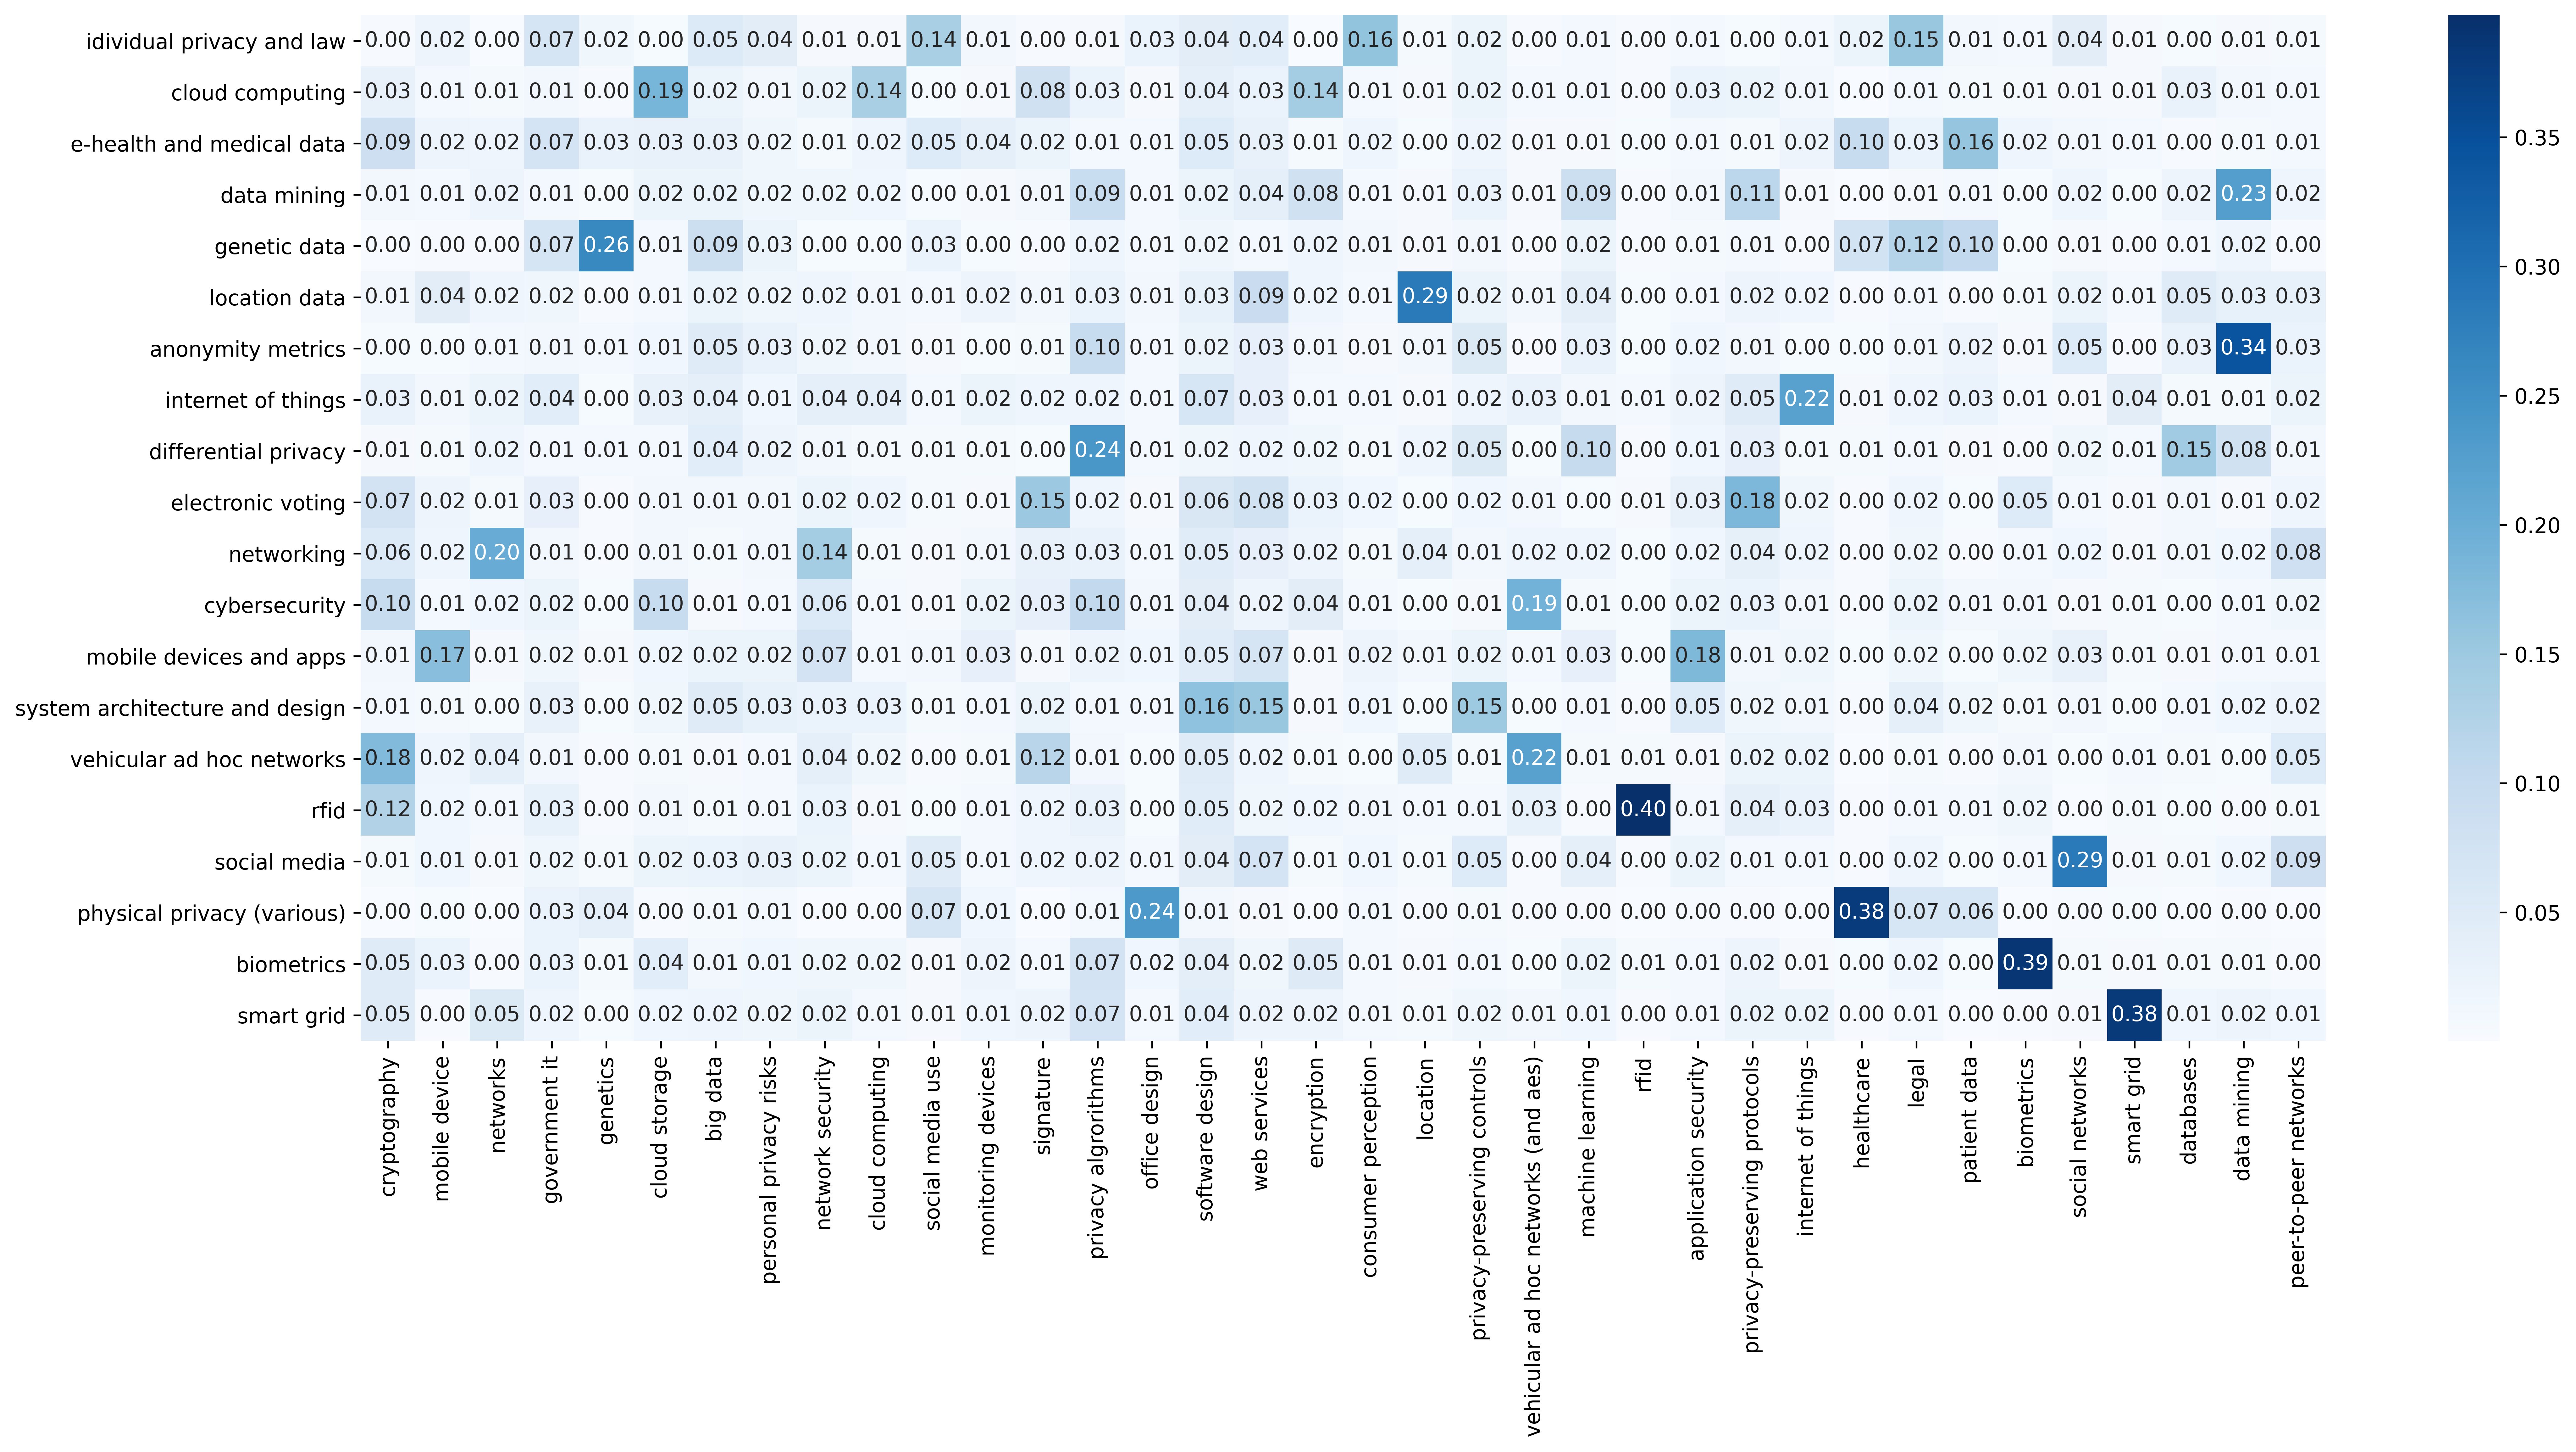
\includegraphics[width = 1\textwidth]{figures/square.png}
    \caption{Average proportion of topic occurrence within network communities}
    \label{fig:square}
\end{figure}

Overall, this overview of relations between the two classifications\footnote{Technically speaking, the topic model does not classify documents into a single category, but we will speak of the `assignment of topic distribution' as a classification for readability purposes} shows some clear patterns. Especially because values close to 1 are impossible since all documents in a community contain multiple topics. Most importantly, it is a remarkable result that two methods that use completely different document properties end up in a relation to each other in which for most of the classifications from the network method, one or multiple counterparts can be clearly distinguished in the topics from the topic model. 

For some communities, there is a clear 1-on-1 relation to one of the topics. Examples are \textit{biometrics}, \textit{RFID}, \textit{smart grid}, \textit{location data} and \textit{genetic data}, for which all papers contained in the community are between 26\% and 40\% 'assigned to' one specific topic. Apparently, these areas of research were equally identifiable with both methods. Some patterns make sense after looking at the citation network. In the network, the communities of \textit{data mining} and \textit{anonymity metrics} are heavily interconnected. Since \textit{anonymity metrics} was not identified as a separate topic by the LDA algorithm, it is not strange to find it to be contained in the topic that was labeled as \textit{data mining}. The fact that \textit{anonymity} is one of the top words in this topic seems to confirm this.

Since the communities are not uniform in size, it is to be expected that the larger communities cover multiple topics. The citation network community of \textit{individual privacy} contains literature 'assigned to' topics on \textit{social media use}, \textit{consumer perception} and \textit{legal} matters. The community of \textit{cloud computing} contains literature on \textit{cloud storage, cloud computing} and \textit{encryption}. Often, the topics that are part of bigger communities are not common as a proportion of other communities; another sign of many similarities between the two classifications. 

On the other hand, some topics are a proportion of many of the communities. This is notably the case for the topics of \textit{software design}, \textit{web services}, \textit{cryptography} and \textit{privacy algorithms}. There are multiple possible explanations: papers on this subject could be very distinctive but widely used in different research areas, or the words related to these subjects could be a smaller part of many papers about different topics. We cannot know whether one or both are mislabeled, nor can we know whether the community or topic was wrongfully identified or uncovered. We will get back to this in the discussion.

\section{Discussion}
\label{discussion}
This paper has explored the usage of an LDA topic model to gain insights into the embedding of privacy in the scientific literature. Firstly, by carefully working out what kind of procedure is needed to create a model that is up to scientific standards and secondly, by comparing it to a different model created on other properties of the literature.

Reflecting on the creation of the topic model, we have to conclude that its full potential is currently limited by the amount of computation time needed. Because we need a grid search to find the `best' model, it is computationally unfeasible to do the type of exploratory research that fits these kinds of creative methods. Ideally, a researcher could easily adjust model parameters and get immediate feedback to `get a feeling' for the model. Being able to look at the multitude of possible topic models is especially important because there is no true value for $N$, the number of topics. Picking just one model for analysis is somewhat arbitrary, and comparing a multitude of models might result in new insights into the scientific discourse.

Observations of just the latent topics did not reveal much insight into the scientific discourse about privacy. Notable associations between topics were often on the method level, distracting from analysis on a higher level. Tweaking the algorithm or relaxing some of the model's assumptions, like the bag-of-words approach, could increase its usefulness. However, doing exploratory research with novel algorithms applied to bibliometric analysis requires a level of mathematical understanding that might be a rare combination with domain knowledge or incentives to perform further research on applications like these.

The second part of the results, where the topic model was compared to a citation network analysis of the same data, showed how two different methods of categorizing literature could result in surprisingly similar results. The fact that so many topics could be related to communities in the citation network is remarkable and gives evidence for a certain extent of both methods' validity. For cases in which the topic-community relation was not one-to-one, this could be explained by differences in size: one community contained multiple topics.

When the two classifications do not match one-to-one, the human capacity to see patterns is lurking. However, we have to be very careful with our interpretation. Combining the two classifications stacks uncertainties of subjectivity when choosing a community detection method, choosing the number of topics, and labeling the communities and topics. When a relationship between a topic and a community is unusual, we can not know whether there is actual meaning to be found behind it. Since, for each observation, the possibility exists that the topic or community was erroneously uncovered, just the coincidental consequence of the chosen method or algorithm parameter, or mislabeled. For scientific rigor, a way to check which of the observed patterns still holds when these factors change would be needed; a sensitivity analysis of conclusions.

Furthermore, the question arises on which level of abstraction the documents are classified. It is challenging to distinguish groupings on the basis of methods as opposed to groupings by subject. Topics showing up as small proportions in several communities leave us wondering whether we uncovered subjects relevant to many disciplines or topics not corresponding to subjects but containing widely used techniques. Additionally, there is still the possibility we are looking at one of the errors mentioned above in our methods, and there is no actual pattern in the literature.

More research into these methods is essential before these novel applications can be more than something to stimulate a discussion and inspire further research. 

\bibliographystyle{splncs04}
\bibliography{bibfile}






\end{document}
